\chapter[This is a long title to check the proper spacing in the
Table of Contents and inverse pyramid on the chapter page. Lets see if it works properly. What if I add enough text so that there are like three or four lines here, does it change the way it looks.]{This is a long title to check the proper spacing in the
Table of Contents and\newline
inverse pyramid on the chapter page. Lets see if it works properly. What if\newline
I add enough text so that there are like three or four lines here,\newline
does it change the way it looks.}



\subsection{A Figure}
Here we have a section to show off one of the xkcd comics. \ref{fig:xkcd1} shows one of the comics showing the actual size of a number compared to the perceived size of a number. 

\begin{figure}[ht]
    \centering
    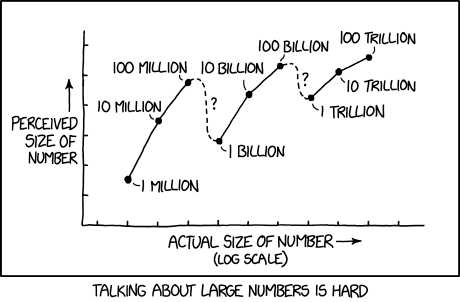
\includegraphics[width=0.7\textwidth]{image-01-million_billion_trillion.png}
    \caption{The trend of actual versus perceived size of a number. \cite{cite-munroe_2018}. We are also
    going to add a relatively long caption to check if the List of Figures works properly at the beginning of the document.}
    \label{fig:xkcd1}
\end{figure}
%Make sure to get permission to include any figures that you did not create, or indicate the open license. See guidelines in C-Appendix.tex

\subsection{Citing and referencing things}
On other figure shown in \ref{fig:phd-Comics1} shows a comic form \cite{cite-cham_2009}. 
If you want to group citations into one go, something you might do in the back ground section, you can do this by grouping multiple sources in your bibtex in the same 'cite' \cite{cite-A,cite-B,cite-C, cite-munroe_2018}.

You can also reference chapter, subsections or appendices al long as you place the label properly. Here I will reference you to see Appendix~\ref{sec:longtable} to check out how to add "longtabes" into your document, another example of that is shown in a hidden chapter on tables.
If you think there was something important in a previous section that you can reference them back with, Section \ref{sec:firstSection}. Or reference a chapter like Chapter \ref{chap:intro}.

Foot notes are allowed depending on the department you are working with. Please check with your advisor if you should be adding foot notes or not. Just so you have an example here is a footnote\footnote{here is a footnote}.

\csmfigure{phd-Comics1}{image-02-phd092809s.png}{5in}{"Vacation Relaxation?" by Jorge Cham
www.phdcomics.com. A nice comic form PHD Comic's. Learn more about the figure input notation in the Figure chapter, or in the hand book.}


Filler Text. \lipsum[4]

\subsection{Here is a test of a really long sub-header title that should automatically follow the rules for set for the Temple Guidelines and check if it properly shows up in the table of content. }

Here is a paragraph of filler text. \lipsum[2]
here is an extra sentence